\chapter{Integração de uma Arquitetura de Transporte QUIC sobre ICE}
\label{chap:implementation}

Este capítulo descreve a implementação da comunicação entre \textit{peers} situados atrás de NATs por meio das técnicas de travessia de NAT apresentadas na Seção~\ref{sec:nat_traversal}. O desenvolvimento se concentra nas etapas de \textit{hole punching} dos métodos baseados em UDP e, em seguida, estende essa comunicação ao protocolo QUIC com a biblioteca \texttt{OpenSSL} \citep{openssl_quic}.

Este trabalho teve origem em um projeto realizado em conjunto com a DATACOM, cujo objetivo era viabilizar a comunicação entre dois \textit{peers} com o mínimo de infraestrutura. Após o encerramento do projeto, o trabalho teve continuidade em caráter acadêmico, no contexto deste TCC.

Inicialmente, o objetivo era transmitir dados TCP, especificamente HTTP, por meio de técnicas de \textit{hole punching}. Devido à complexidade do \textit{hole punching} TCP (Seção~\ref{sec:tcp_hole_punching}), optou-se pelo \textit{hole punching} UDP. A base adotada foi o Chownat, que, além de realizar \textit{hole punching}, tunela dados TCP sobre UDP sem transmitir os pacotes de controle do TCP, permitindo uma comunicação direta entre os \textit{peers}.

Para a comunicação, o projeto propôs um servidor mínimo (\textit{rendezvous server}), responsável pela autenticação e pela troca de endereços IP entre os \textit{peers}, com função semelhante à de um servidor STUN na descoberta de endereços. O projeto também propôs um protocolo capaz de atender aos requisitos de dependabilidade e segurança descritos na introdução deste trabalho. O protocolo escolhido foi o QUIC, devido à sua adoção crescente e à sua compatibilidade com os requisitos de transmissão de dados de aplicação do projeto.

O projeto implementou apenas parcialmente a infraestrutura de servidores e avançou pouco na comunicação QUIC entre dois \textit{peers}. Este trabalho também estende o trabalho de \citet{paladin2025quic}, que abordou os aspectos de segurança e as razões para a escolha do QUIC nos cenários propostos.

A implementação descrita neste capítulo executa nos \textit{gateways} da arquitetura proposta, que realizam a comunicação externa e executam as aplicações integradas ao túnel. O objetivo é interligar essas aplicações quando os \textit{gateways} se encontram em redes distintas, por meio dos mecanismos de descoberta e seleção de caminhos da solução. Os dispositivos IoT, como sensores e atuadores, não participam da negociação de conectividade, e a obtenção e o encaminhamento de seus dados cabem à aplicação do \textit{gateway}. Nos experimentos, aplicações locais de geração e recepção de mensagens representam esses dados. Nos ambientes de teste, os \textit{gateways} correspondem a \textit{hosts} de propósito geral, e os roteadores da topologia realizam o encaminhamento de pacotes e, quando configurados para isso, a tradução de endereços (NAT). A implementação não é executada nesses roteadores. Este trabalho também não estabelece requisitos mínimos de execução nem caracteriza o consumo das bibliotecas utilizadas em dispositivos IoT com recursos limitados.

A Figura~\ref{fig:chapter_structure} apresenta a organização do capítulo. À esquerda, a figura mostra as camadas da implementação executada nos \textit{gateways}. À direita, mostra os ambientes utilizados na avaliação. Cada bloco indica a seção que o descreve.

A Seção~\ref{sec:hole_punching_protocols} apresenta a tradução e a extensão do protocolo Chownat (Seção~\ref{sec:chownat}), a interface genérica de \textit{hole punching} (\texttt{udp\_conn}) derivada desse protocolo e a implementação QUIC baseada na biblioteca \texttt{OpenSSL}. A Seção~\ref{sec:ice_library} generaliza a solução com o ICE. Nessa etapa, a interface \texttt{udp\_transport} abstrai o \textit{socket} UDP, e a biblioteca \texttt{libnice} assume a obtenção de candidatos, o \textit{hole punching} e o gerenciamento dos \textit{sockets}, tanto para protocolos genéricos, como o Chownat, quanto para a OpenSSL. Por fim, a Seção~\ref{sec:topologies} apresenta as topologias de teste, e a Seção~\ref{sec:simulation_environments} descreve os ambientes experimentais, compostos por dois ambientes de simulação e uma infraestrutura física.

\begin{figure}[ht]
\centering
% Estrutura do Capítulo~\ref{chap:implementation} (Figura~\ref{fig:chapter_structure})
% Requer: \usepackage{tikz} e \usetikzlibrary{positioning,fit,arrows.meta,calc}
\resizebox{0.8\textwidth}{!}{%
\begin{tikzpicture}[
  font=\sffamily\small,
  >={Stealth[length=2.2mm]},
  layer/.style={draw, rounded corners=2pt, minimum height=11mm, align=center, inner sep=3pt},
  app/.style={layer, fill=gray!12},
  ifc/.style={layer, fill=blue!10},
  proto/.style={layer, fill=green!10},
  trans/.style={layer, fill=orange!14},
  env/.style={layer, fill=violet!8},
  group/.style={draw=black!45, dashed, rounded corners=4pt, inner sep=7pt},
  title/.style={font=\sffamily\small\bfseries}
]
\def\figsr#1{\\[-1pt]{\scriptsize\itshape Seção~\ref{#1}}}
% ---------------- Implementação no gateway ----------------
\node[app, minimum width=80mm] (app) {Aplicação local sobre TCP (HTTP, MQTT, \ldots)\figsr{sec:tcp_tunneling}};
\node[ifc, minimum width=80mm, below=4mm of app] (udpconn)
  {\texttt{udp\_conn}: interface de \textit{hole punching}\\[-1pt]
   \scriptsize tunelamento TCP $\cdot$ API e \textit{loop} de eventos\figsr{sec:hole_punching_interface}};
\node[proto, minimum width=38mm, below=4mm of udpconn.south west, anchor=north west] (chownat)
  {Chownat traduzido\\[-1pt]\scriptsize e estendido\figsr{sec:chownat_translation_extension}};
\node[proto, minimum width=38mm, below=4mm of udpconn.south east, anchor=north east] (ossl)
  {\texttt{ossl\_quic}\\[-1pt]\scriptsize QUIC da \texttt{OpenSSL}\figsr{sec:ossl_quic_for_hole_punching}};
\node[proto, minimum width=38mm, below=4mm of ossl, fill=green!5] (bio)
  {BIO personalizado\figsr{sec:openssl_bio}};
\node[trans, minimum width=80mm, below=4mm of bio.south east, anchor=north east] (udptr)
  {\texttt{udp\_transport}: gerência do \textit{socket} UDP\figsr{sec:udp_transport}};
\node[trans, minimum width=38mm, below=4mm of udptr.south west, anchor=north west] (direct)
  {\textit{Direct UDP}\\[-1pt]\scriptsize abordagem legada\figsr{sec:hole_punching_interface}};
\node[trans, minimum width=38mm, below=4mm of udptr.south east, anchor=north east] (ice)
  {ICE com \texttt{libnice}\\[-1pt]\scriptsize STUN $\cdot$ TURN $\cdot$ sinalização\figsr{sec:libnice_integration}};
\node[layer, minimum width=80mm, below=4mm of direct.south west, anchor=north west, fill=white] (net)
  {Rede com NAT\figsr{sec:nat_traversal}};

\draw[->] (app) -- (udpconn);
\draw[->] (udpconn.south -| chownat) -- (chownat);
\draw[->] (udpconn.south -| ossl) -- (ossl);
\draw[->] (ossl) -- (bio);
\draw[->] (chownat) -- (chownat |- udptr.north);
\draw[->] (bio) -- (bio |- udptr.north);
\draw[->] (udptr.south -| direct) -- (direct);
\draw[->] (udptr.south -| ice) -- (ice);
\draw[->] (direct) -- (direct |- net.north);
\draw[->] (ice) -- (ice |- net.north);

\node[group, fit=(app)(net)(udpconn)(ice)] (stack) {};
\node[title, anchor=south west] at (stack.north west) {Implementação no \textit{gateway} {\mdseries\scriptsize (Seções~\ref{sec:hole_punching_protocols} e~\ref{sec:ice_library})}};

% ---------------- Ambientes de avaliação ----------------
\node[env, minimum width=26mm, right=24mm of udpconn.east, anchor=west, yshift=6mm] (tdir)
  {Topologia\\[-1pt]\scriptsize direta\figsr{sec:basic_topology_hole_punching}};
\node[env, minimum width=26mm, right=3mm of tdir] (tice)
  {Topologia\\[-1pt]\scriptsize ICE\figsr{sec:ice_topology}};
\node[env, minimum width=55mm, anchor=north west] (gns3) at ($(tdir.south west)+(0,-9mm)$)
  {GNS3\\[-1pt]\scriptsize uso inicial, sem resultados\figsr{sec:gns3}};
\node[env, minimum width=55mm, below=3mm of gns3] (ns)
  {\textit{Linux Network Namespaces}\\[-1pt]\scriptsize com PatchBay\figsr{sec:linux_network_namespaces}};
\node[env, minimum width=55mm, below=3mm of ns] (phy)
  {Infraestrutura física (DATACOM)\figsr{sec:physical_infrastructure}};
\node[font=\sffamily\scriptsize\bfseries, anchor=south] at (gns3.north) {Ambientes (Seção~\ref{sec:simulation_environments})};
\node[font=\sffamily\scriptsize\bfseries, anchor=south] at ($(tdir.north)!0.5!(tice.north)$) {Topologias (Seção~\ref{sec:topologies})};

\node[group, fit=(tdir)(tice)(phy), inner ysep=14pt] (eval) {};
\node[title, anchor=south west] at (eval.north west) {Ambientes de avaliação};

\draw[->, thick, black!60] (stack.east |- ns) -- node[above, font=\sffamily\scriptsize] {validação} (eval.west |- ns);
\draw[->, thick, black!60] (eval.south) -- ++(0,-7mm) node[below, font=\sffamily\scriptsize] {Resultados: Capítulo~\ref{chap:results}};
\end{tikzpicture}%
}

\caption{Estrutura do capítulo: camadas da implementação executada nos \textit{gateways} e ambientes utilizados na avaliação, com as seções correspondentes.}
\label{fig:chapter_structure}
\end{figure}

\section{Protocolos de Comunicação para Hole Punching}
\label{sec:hole_punching_protocols}

Esta seção apresenta as implementações e extensões desenvolvidas para viabilizar a comunicação com as técnicas de \textit{hole punching} propostas inicialmente, o que permite a comunicação direta entre dois \textit{peers} situados atrás de NATs:

\begin{itemize}
    \item a Seção~\ref{sec:chownat_translation_extension} apresenta a tradução e a extensão do Chownat, iniciadas durante o projeto com a DATACOM;
    \item a Seção~\ref{sec:hole_punching_interface} apresenta a interface de transporte genérica para \textit{hole punching}, derivada do Chownat;
    \item a Seção~\ref{sec:ossl_quic_for_hole_punching} apresenta uma proposta de uso da biblioteca OpenSSL no modo \textit{threadless} para \textit{hole punching}.
\end{itemize}

\subsection{Tradução e Extensão do Protocolo Chownat}
\label{sec:chownat_translation_extension}

O Chownat foi implementado originalmente em Perl \citep{kamkar2004chownatv07}. O projeto com a DATACOM, descrito no início deste capítulo, adotou esse protocolo porque ele atendia às necessidades iniciais de compreensão e aplicação de técnicas de travessia de NAT. Além disso, o protocolo realiza \textit{hole punching} de forma nativa e oferece tunelamento TCP, necessário ao tráfego das aplicações HTTP do projeto.

Durante o projeto, o protocolo foi traduzido para C e Dart, com a preservação de seu funcionamento original, sem extensões nem modificações. Essa tradução, entretanto, estava incompleta e apresentava diversas limitações, principalmente nas etapas de criação, reinício e finalização de conexões. Além disso, como o Chownat foi concebido apenas para tunelamento TCP, não era possível uma comunicação somente com UDP.

Embora não constituam o objetivo principal deste trabalho, as extensões e modificações no Chownat permitiram testar o funcionamento da interface (Seção~\ref{sec:hole_punching_interface}) e generalizá-la para protocolos posteriores, como o QUIC. Portanto, o valor desse desenvolvimento está na verificação do funcionamento, e não na recomendação do protocolo para outras aplicações. O Chownat apresenta diversas limitações, como a falta de garantia dos requisitos de dependabilidade, citados na introdução deste trabalho, que são essenciais na transmissão de dados IoT.

\subsubsection{Limitações do Chownat e Extensões Desenvolvidas}
\label{sec:chownat_limitations}

O Chownat possui diversas limitações, associadas principalmente ao seu objetivo original. Na época de seu desenvolvimento, em 2004 \citep{kamkar2004chownat}, as técnicas de travessia de NAT ainda estavam em exploração, e as arquiteturas de rede P2P eram vistas com desconfiança, devido à sua associação com a pirataria. Assim, o Chownat não parece ter sido concebido para uso contínuo em um dispositivo, mas sim para demonstrar o funcionamento de técnicas de \textit{hole punching} em dispositivos NAT.

Como a interface genérica, apresentada na Seção~\ref{sec:hole_punching_interface}, se baseia no Chownat, os mecanismos propostos para generalizá-la e viabilizar seu uso por outros protocolos também beneficiam o próprio Chownat. Algumas limitações não foram solucionadas, principalmente as específicas do protocolo, como suas garantias de dependabilidade. Ainda assim, parte delas foi resolvida para permitir testes sobre os recursos da interface. As principais limitações e o tratamento dado a cada uma são:

\begin{itemize}
    \item \textbf{Conexão suporta apenas o envio de 256 pacotes:} o identificador de pacote ocupa um único byte e, portanto, assume valores entre 0 e $2^8-1$. Optou-se por manter o cabeçalho do Chownat (Seção~\ref{sec:chownat_protocol}) e reiniciar a contagem ao atingir o limite. Perdas de mais de 256 pacotes consecutivos ainda geram comportamento indefinido, mas essa solução foi preferida à extensão do campo para 2 bytes, pois preserva o formato original do pacote;
    \item \textbf{Apenas permite comunicação de dados TCP:} o Chownat funciona apenas com tunelamento TCP e não permite o envio nativo de dados UDP. Com a interface genérica, o tunelamento TCP passou a ser opcional por conexão, e a aplicação pode enviar dados nativamente, sem depender de uma conexão TCP externa;
    \item \textbf{Permite apenas uma conexão por aplicação:} ao finalizar a única conexão TCP suportada, o protocolo original entrava em \textit{loop} infinito. A solução consistiu em implementar um \textit{3-way handshake} de desconexão, com número máximo de tentativas configurável por conexão. Assim, ao finalizar uma conexão TCP, a conexão Chownat também é finalizada, e uma nova conexão pode ser inicializada;
    \item \textbf{Hole punching exige tradução de porta com ``mapeamento espelhado'':} o \textit{hole punching} do Chownat depende de o NAT preservar a porta de origem, isto é, mapear o tráfego para a mesma porta à qual o \textit{socket} remetente está vinculado. Alguns NATs apresentam esse comportamento, como o NAT simulado pelo PatchBay \citep{patchbay} no modo \textit{Moderate}, mas trata-se de um caso particular, e não de uma regra geral entre implementações de NAT. A integração da biblioteca ICE, descrita na Seção~\ref{sec:ice_library}, resolveu posteriormente esse problema;
    \item \textbf{Sem garantias de dependabilidade:} o protocolo não oferece garantias de confiabilidade, integridade, autenticidade ou segurança. Essa limitação não foi resolvida, pois o objetivo final é o uso do QUIC, que oferece nativamente entrega confiável e proteção criptográfica. Manteve-se, portanto, a simplicidade do Chownat para fins exclusivos de teste.
\end{itemize}

Em síntese, as extensões desenvolvidas não tornam o Chownat um protocolo pronto para uso em produção. Sua limitação mais fundamental, a ausência de garantias de dependabilidade, foi deliberadamente mantida. O valor desse trabalho de extensão está em fornecer um protocolo funcional e conhecido como base de testes para a interface genérica, o que permitiu validar empiricamente as técnicas de \textit{hole punching} antes de aplicá-las a um protocolo com garantias mais robustas, como o QUIC.

\subsection{Interface de Transporte para Hole Punching}
\label{sec:hole_punching_interface}

A interface de transporte para \textit{hole punching} foi criada especificamente para este trabalho, com o objetivo de permitir que múltiplos protocolos de transporte sobre UDP realizem \textit{hole punching}, independentemente de o protocolo oferecer esse recurso nativamente. A interface também habilita o tunelamento de TCP sobre esses protocolos, permitindo transportar dados de serviços da camada de aplicação baseados em TCP por meio de outros protocolos de transporte.

A interface é baseada no Chownat (Seção~\ref{sec:chownat}) e propõe uma versão modular desse protocolo, cuja estrutura pode ser reutilizada na aplicação de \textit{hole punching} a outros protocolos, como o QUIC. O objetivo principal é reutilizar os componentes do protocolo original, isto é, as partes associadas ao \textit{hole punching} e ao tunelamento TCP, de modo que a integração de outro protocolo exija apenas a substituição de componentes.

A interface também adota uma abordagem \textit{threadless}, com uma API baseada em eventos inspirada na API da biblioteca \texttt{libwebsockets} \citep{libwebsockets}. Essa implementação utiliza a chamada de sistema \texttt{select}, que monitora múltiplos \textit{sockets} e aguarda a chegada de novos dados em qualquer um deles.

Além disso, a interface oferece um modelo de configuração que gerencia o uso do \textit{hole punching} e do tunelamento TCP. Essa configuração ocorre antes do início da conexão do protocolo, o que também favorece a arquitetura modular.

\subsubsection{Configuração da Interface}

Assim como o Chownat, a interface mantém duas sessões, uma UDP e outra TCP, o que permite o tunelamento.

Cada sessão possui configurações próprias, como \textit{timeouts} e endereços de origem e destino. Assim, uma aplicação pode configurar a interface previamente a partir de dados obtidos externamente, por exemplo, por meio do ICE.

A configuração também permite registrar uma função de \textit{callback}, chamada a cada novo evento com o motivo (\textit{reason}) do evento como parâmetro.

Para fornecer uma organização baseada no paradigma de orientação a objetos, a configuração permite escolher a implementação de protocolo que utilizará a sessão UDP. Um novo protocolo UDP precisa apenas implementar um conjunto de funções predefinidas, de forma análoga a uma tabela de métodos virtuais (\textit{vtable}). Na prática, essa tabela corresponde a um conjunto de ponteiros de função que cada implementação de protocolo deve fornecer. A Figura~\ref{fig:udp_conn_diagram} apresenta o diagrama de blocos da API pública da interface.

\begin{figure}[ht]
    \centering
    \includegraphics[width=0.8\textwidth]{fig/implementation/interface/udp_conn_diagram.png}
    \caption{Diagrama de blocos da interface genérica de conexão UDP udp\_conn.}
    \label{fig:udp_conn_diagram}
\end{figure}

A interface genérica permite ainda que o protocolo UDP opere em dois modos, cliente e servidor. Cada modo executa funções específicas no uso do tunelamento TCP. Esses comportamentos correspondem aos descritos na Seção~\ref{sec:chownat} e são detalhados na Seção~\ref{sec:interface_connection_flow_and_hole_punching}.

\subsubsection{Fluxo de Conexão e Hole Punching}
\label{sec:interface_connection_flow_and_hole_punching}

A conexão por meio desta interface se baseia em três operações, cuja ordem define se o processo opera como cliente ou como servidor. As operações são as seguintes:

\begin{enumerate}
    \item \textbf{Bind TCP:} vincula a sessão TCP ao serviço local;
    \item \textbf{Hole Punching:} realiza a travessia de NAT por \textit{hole punching} UDP;
    \item \textbf{Conexão UDP:} executa o processo de conexão do próprio protocolo, quando este não está integrado ao \textit{hole punching}.
\end{enumerate}

Para compreender essas diferenças, é preciso retomar as etapas de conexão descritas na Seção~\ref{sec:chownat_connection}. No modo cliente, a interface aguarda uma conexão TCP de outro processo da própria máquina destinada ao serviço desejado. No modo servidor, a interface aguarda apenas uma conexão UDP remota. Após receber a conexão TCP local, o cliente inicia o \textit{hole punching}. O servidor, por sua vez, conecta-se ao serviço TCP local somente após concluir o \textit{hole punching}. Assim, as duas operações ocorrem em ordem inversa nos dois modos, o que gera o fluxo da Figura~\ref{fig:udp_conn_connection_flow_diagram}.

\begin{figure}[ht]
    \centering
    \includegraphics[width=0.8\textwidth]{fig/implementation/interface/udp_conn_connection_flow_diagram.png}
    \caption{Diagrama de tempo da interface de conexão UDP \texttt{udp\_conn}.}
    \label{fig:udp_conn_connection_flow_diagram}
\end{figure}

A implementação do protocolo UDP é responsável apenas pelas etapas de comunicação externa com o outro \textit{peer}. A própria interface gerencia as comunicações TCP internas, de modo que o protocolo não precisa conhecer o funcionamento do tunelamento.

\subsubsection{API e Loop de Eventos}
\label{sec:api_and_event_loop}

A API baseada em eventos é uma adição ao Chownat que permite um comportamento reativo e o uso do protocolo sem tunelamento TCP. Essa API integra a extensão do Chownat descrita na Seção~\ref{sec:chownat_translation_extension}.

A interface recebe eventos em dois níveis. O primeiro corresponde aos eventos que o sistema operacional sinaliza à interface quando um novo pacote chega a um \textit{socket}. A chamada de sistema \texttt{select} aguarda atividade em um subconjunto de \textit{sockets} e retorna quando há dados ou quando o tempo limite expira, o que permite à interface continuar a execução. O Chownat já utilizava essa chamada, e o tempo limite do \texttt{select} determina o envio periódico de pacotes \textit{keep-alive}, que abrem e mantêm os mapeamentos nos NATs (Listagem~\ref{lst:select_pseudocode}).


\begin{lstlisting}[float=htbp, caption={Pseudocódigo do loop de eventos da interface}, label={lst:select_pseudocode}]
    while (true)
        ret = select(sockets, ..., timeout)
        if (ret == TIMEOUT_EXCEEDED)
            send_keep_alive()
        else
            handle_sockets()
\end{lstlisting}

O segundo nível corresponde aos eventos entregues à aplicação. Cada implementação de protocolo define seus próprios eventos, como o recebimento de uma mensagem, a ocorrência de um erro e o início ou o fim de uma conexão. Por meio desses eventos, a aplicação pode intervir no fluxo de conexão com a API pública da interface, que inclui as seguintes ações:

\begin{itemize}
    \item \textbf{udp\_conn\_send:} envia uma mensagem;
    \item \textbf{udp\_conn\_recv:} aguarda o recebimento de uma mensagem;
    \item \textbf{udp\_conn\_disconnect:} finaliza a conexão.
\end{itemize}

Além dessa API pública, a interface oferece funções de criação e finalização de conexão, que não podem ser chamadas dentro do \textit{loop} de eventos:

\begin{itemize}
    \item \textbf{udp\_conn\_init:} inicializa a interface com uma implementação de protocolo;
    \item \textbf{udp\_connection:} inicializa a conexão e executa o próprio \textit{loop} de eventos, do qual retorna somente quando a conexão é finalizada;
    \item \textbf{udp\_conn\_deinit:} desinicializa a interface.
\end{itemize}

\subsubsection{Tunelamento TCP}
\label{sec:tcp_tunneling}

O tunelamento TCP é um dos principais atributos da arquitetura do Chownat. Ele permite a conectividade entre \textit{peers} e o reuso de serviços implementados sobre TCP, com menor \textit{overhead} de comunicação. Ele também contribui para a modularidade dos serviços, pois desacopla indiretamente o protocolo de transporte, e facilita a migração de serviços baseados em TCP para UDP. Essa facilidade de migração é relevante para a proposta deste trabalho, devido à ampla utilização, na Internet das Coisas (IoT), de protocolos de aplicação baseados em TCP e em arquiteturas cliente-servidor, como HTTP e MQTT. Assim, a solução proposta busca facilitar a adoção de uma arquitetura \textit{peer-to-peer} por aplicações existentes, com menos modificações nos serviços desenvolvidos originalmente para TCP.

A interface oferece o tunelamento de forma transparente à implementação do protocolo, como um recurso opcional para a aplicação. Conforme a Seção~\ref{sec:chownat}, a conexão TCP ocorre apenas localmente. O serviço envia seus pacotes à interface por meio de um \textit{socket} TCP vinculado a ele, de modo que os segmentos de controle TCP (como SYN, ACK e FIN) permanecem locais e a conexão remota transporta apenas os dados do serviço de aplicação (HTTP, SSH etc.). O protocolo sobre UDP, entretanto, pode transmitir seus próprios pacotes de controle. Quando a aplicação envia uma mensagem ao \textit{socket} vinculado, o \textit{loop} de eventos da interface (Seção~\ref{sec:api_and_event_loop}) sinaliza o recebimento, e a interface identifica o \textit{socket} de origem. Se os dados chegam pelo \textit{socket} TCP, a interface os encaminha pela implementação UDP. Se chegam pela implementação UDP, o protocolo apenas os entrega à interface, que verifica se há tunelamento ativo e os redireciona ao \textit{socket} TCP local, o que permite a resposta à aplicação. A Figura~\ref{fig:udp_conn_tcp_tunneling_diagram} apresenta esse fluxo completo.

\begin{figure}[ht]
    \centering
    \includegraphics[width=1.0\textwidth]{fig/implementation/interface/udp_conn_tcp_tunneling_diagram.png}
    \caption{Diagrama de tempo de uma requisição TCP tunelada por UDP utilizando a interface udp\_conn.}
    \label{fig:udp_conn_tcp_tunneling_diagram}
\end{figure}

\subsection{Uso da Biblioteca OpenSSL para QUIC Hole Punching}
\label{sec:ossl_quic_for_hole_punching}

Devido à complexidade do QUIC (Capítulo~\ref{chap:quic}), optou-se por utilizar uma biblioteca para a comunicação entre \textit{peers} com esse protocolo. Além disso, o protocolo incorpora diversos mecanismos de segurança, o que desaconselha uma implementação própria, sujeita a riscos decorrentes de falhas de implementação.

Como o objetivo é utilizar uma arquitetura baseada no Chownat, este trabalho não adota implementações existentes de \textit{QUIC hole punching}, pois elas seguem abordagens diferentes, como alterações no próprio protocolo QUIC, a exemplo da segunda proposta de \citet{draft-seemann-quic-nat-traversal}. O objetivo foi utilizar uma biblioteca consolidada para implementar a primeira alternativa de \textit{QUIC hole punching} proposta por \citet{draft-seemann-quic-nat-traversal}, que consiste em realizar o \textit{hole punching} previamente, via ICE ou método equivalente, e então estabelecer a conexão QUIC sobre o caminho já aberto.

Para a implementação do QUIC, optou-se pela biblioteca \texttt{OpenSSL}, um projeto de código aberto consolidado no desenvolvimento de soluções criptográficas e protocolos de comunicação segura. A partir da versão 3.2, lançada em novembro de 2023 \citep{openssl_quic}, a \texttt{OpenSSL} passou a oferecer suporte nativo a conexões QUIC no lado cliente, e a versão 3.5 estendeu esse suporte ao lado servidor. A escolha se fundamenta na manutenção ativa do projeto, na disponibilidade de documentação oficial e na integração do QUIC à API SSL existente, que permite reutilizar abstrações e mecanismos de comunicação da biblioteca. Além disso, a \texttt{OpenSSL} aceita um \textit{socket} externo, o que permite reutilizar um \textit{socket} que já passou por \textit{hole punching} e manter o caminho aberto para a conexão QUIC. Esse recurso é um pré-requisito para combinar a arquitetura do Chownat com a primeira alternativa de \citet{draft-seemann-quic-nat-traversal}, que não altera o protocolo.

\subsubsection{Configuração e Conexão do Protocolo QUIC}

A implementação do protocolo sobre a interface expõe apenas parte da API da \texttt{OpenSSL} e funciona como um \textit{wrapper}, que adiciona configurações para simplificar o uso. Esse \textit{wrapper} recebeu o nome ``ossl\_quic''. O usuário pode configurar, no cliente e no servidor, as suítes criptográficas do TLS 1.3 disponibilizadas pela \texttt{OpenSSL}, pois o QUIC utiliza exclusivamente o TLS 1.3 em seu \textit{handshake}.

A \texttt{OpenSSL} organiza suas configurações em contextos. As configurações de cliente e servidor diferem principalmente porque este trabalho não utiliza o mTLS (\textit{mutual TLS}), que autentica tanto o servidor quanto o cliente. Nos experimentos, o servidor utilizou um certificado autoassinado, e a validação do certificado pelo cliente foi desabilitada. Essa configuração estabelece uma conexão cifrada, mas não verifica a identidade do servidor remoto. Seu uso se restringiu aos testes. Em produção, a validação do certificado deve estar habilitada, com uma configuração de confiança adequada para verificar a identidade do servidor remoto.

Além disso, embora não tenha sido abordado no Capítulo~\ref{chap:quic}, o QUIC exige a negociação do protocolo de aplicação por meio da extensão ALPN (\textit{Application Layer Protocol Negotiation}) durante o \textit{handshake}. Como o objetivo é transportar dados genéricos, não associados a um protocolo de aplicação específico, utiliza-se um identificador arbitrário, ``osslquic'', configurado nas duas extremidades.

Assim como no Chownat (Seção~\ref{sec:chownat}), esta etapa inicializa o \textit{socket} UDP e o vincula a um endereço específico. A Figura~\ref{fig:ossl_quic_configuration} apresenta o diagrama de tempo dessa configuração.

\begin{figure}[ht]
    \centering
    \includegraphics[width=0.8\textwidth]{fig/implementation/ossl_quic/ossl_quic_configuration_time_diagram.png}
    \caption{Diagrama de tempo da configuração do QUIC da OpenSSL sobre a interface.}
    \label{fig:ossl_quic_configuration}
\end{figure}

\subsubsection{Processo de Hole Punching e Conexão}

O processo de \textit{hole punching} da implementação ``ossl\_quic'' segue o padrão do Chownat: o \textit{hole punching} ocorre antes da conexão QUIC, o que implementa parcialmente a primeira proposta de \citet{draft-seemann-quic-nat-traversal}. Na prática, esse \textit{hole punching} pode ser realizado pelo próprio ICE, como descrito na Seção~\ref{sec:ice_library}.

Concluído o \textit{hole punching}, inicia-se a conexão QUIC. Essa etapa corresponde à operação opcional de conexão UDP descrita na Seção~\ref{sec:interface_connection_flow_and_hole_punching} e ilustrada na Figura~\ref{fig:udp_conn_connection_flow_diagram}. Antes dela, a implementação executa uma operação interna, denominada neste trabalho \textit{pre connect}. Os datagramas residuais do \textit{hole punching} não exigem descarte manual. O RFC~9000 determina que o servidor descarte pacotes \texttt{Initial} contidos em datagramas UDP com menos de 1200 bytes \citep{rfc9000}, e datagramas que não formam pacotes QUIC válidos também são descartados pela implementação.

A \textit{pre connect}, como o nome indica, ocorre antes da conexão e cria uma nova conexão SSL, nome dado às conexões da \texttt{OpenSSL}, posteriormente utilizada na conexão QUIC. Essa operação cria a conexão, ou o \textit{listener} no caso do servidor, inicializa esse objeto no estado adequado e vincula o descritor de arquivo (\textit{file descriptor}, FD) correspondente, configurando o cliente como conexão e o servidor como \textit{listener}. No lado do cliente, a operação também chama a função POSIX \texttt{connect}, que associa o \textit{socket} UDP a um endereço remoto sem estabelecer uma conexão, ao contrário do que ocorre no TCP. No lado do servidor, o \textit{socket} é configurado inicialmente como bloqueante, para que o servidor aguarde a conexão QUIC.

Durante a conexão, o servidor apenas aguarda, por meio de \texttt{accept}, a chegada de uma conexão externa. O cliente, por sua vez, inicia a conexão por meio da \texttt{OpenSSL}, que executa as etapas descritas na Seção~\ref{sec:quic_connection_steps}.

\subsubsection{Gerência da Conexão}

A gerência da conexão segue o modelo do Chownat (Seção~\ref{sec:chownat}), com o uso de \textit{keep-alives}, o envio e o recebimento de mensagens por meio das chamadas \texttt{send} e \texttt{recv} e a gerência do tunelamento TCP discutida anteriormente. Como a \textit{engine} QUIC da \texttt{OpenSSL} é mais elaborada que um protocolo simples como o Chownat, foi necessário estender a interface da Seção~\ref{sec:hole_punching_interface} para suportar comportamentos da implementação do protocolo. A extensão incluiu o processamento de eventos e o processamento de dados pendentes do protocolo.

O processamento de eventos é necessário porque a interface é \textit{threadless} (Seção~\ref{sec:hole_punching_interface}). Assim, a própria interface precisa processar explicitamente eventos assíncronos, como \textit{timeouts} e o envio e o recebimento de pacotes de controle. Segundo a documentação da \texttt{OpenSSL} \citep{openssl_ssl_handle_events}, esse processamento não seria necessário no modo de assistência por \textit{threads}, no qual uma \textit{thread} interna da biblioteca trata esses eventos periodicamente. As chamadas de \textit{read} e \textit{write} também processam esses eventos e operam em modo bloqueante apenas durante a etapa de conexão. Ainda assim, quando essas chamadas ocorrem em intervalos longos, a interface precisa tratar os eventos explicitamente.

O processamento de dados pendentes, por sua vez, decorre de um comportamento da \texttt{OpenSSL}. Ao receber pacotes QUIC, seja no processamento de eventos, seja em operações de \textit{read}, a biblioteca os armazena em um \textit{buffer} interno. Os dados pendentes passam então a ser lidos da biblioteca, e não mais do \textit{socket}. No Chownat, a espera por dados dependia apenas da existência de dados no \textit{socket}, verificada pelo \textit{loop} de eventos. Com a biblioteca QUIC, essa lógica se torna insuficiente, pois o \textit{socket} aparece vazio assim que a \texttt{OpenSSL} o esvazia internamente, mesmo que pacotes recebidos permaneçam no \textit{buffer} da biblioteca à espera de processamento. Por isso, a interface também precisa processar esses dados pendentes.

Além disso, o processamento de eventos introduz uma segunda dependência temporal na interface. Antes, a única dependência temporal era o \textit{timeout} de atividade nos \textit{sockets}, controlado pela chamada de sistema \texttt{select}. Com a extensão, a \texttt{OpenSSL} passa a definir também um \textit{timeout} para eventos internos. Por isso, o tempo de espera do \texttt{select} pode precisar ser mais curto, para que um evento interno do protocolo seja tratado antes do próximo \textit{keep-alive}.

A solução consiste em manter um ponto de referência de inatividade, atualizado a cada atividade no \textit{socket}. A cada iteração, a interface compara os dois \textit{timeouts} e utiliza o menor como tempo de espera do \texttt{select}. Quando o \texttt{select} expira, a interface verifica se o ponto de inatividade foi atingido. Em caso afirmativo, o \textit{timeout} decorreu da inatividade, e a interface envia um \textit{keep-alive} para manter o mapeamento no NAT. Caso contrário, o \textit{timeout} decorreu do \textit{timeout} interno de eventos, mais curto. Nesse caso, o \textit{loop} retorna ao início e processa os eventos e os pacotes pendentes antes de aguardar o próximo pacote no \texttt{select}.

Dessa forma, o fluxo da Figura~\ref{fig:udp_conn_tcp_tunneling_diagram} recebe alterações que o tornam portável para bibliotecas com requisitos que o Chownat, devido à sua simplicidade, não exigia nem tratava. A Figura~\ref{fig:udp_conn_additional_methods} apresenta o fluxo resultante.

\begin{figure}[!ht]
    \centering
    \includegraphics[width=0.8\textwidth]{fig/implementation/ossl_quic/new_udp_conn_diagram.png}
    \caption{Diagrama de atividades do fluxo atualizado da interface \texttt{udp\_conn}.}
    \label{fig:udp_conn_additional_methods}
\end{figure}

\section{Uso da Biblioteca libnice para a Integração do Protocolo ICE}
\label{sec:ice_library}

Conforme a Seção~\ref{sec:ice}, o ICE é o protocolo responsável por descobrir os endereços candidatos de cada \textit{peer} e selecionar um par de candidatos que permita a comunicação P2P por meio de técnicas de travessia de NAT. A implementação descrita na Seção~\ref{sec:hole_punching_protocols} herda do Chownat a necessidade de conhecer previamente esses endereços. Essa necessidade impõe a dependência do ``mapeamento espelhado'', descrita na Seção~\ref{sec:chownat_limitations}. Para solucionar esse problema de forma genérica, tanto para o Chownat quanto para os protocolos que utilizam a interface \texttt{udp\_conn} (Seção~\ref{sec:hole_punching_interface}), este trabalho criou uma nova interface de transporte, responsável pela gerência do \textit{socket} UDP da conexão. Essa interface permite à aplicação escolher o modelo de transporte, com suporte tanto à abordagem legada da Seção~\ref{sec:hole_punching_interface} quanto à nova abordagem baseada em ICE, descrita nesta seção.

Entre as principais bibliotecas de ICE, este trabalho escolheu a \texttt{libnice} \citep{libnice}, principalmente pela praticidade de integração. A biblioteca oferece uma API baseada em eventos sobre a \texttt{GLib} e implementa os clientes STUN e TURN, que ficam abstraídos da aplicação. Além disso, a \texttt{libnice} é implementada em C, o que facilita a integração direta com sua API. A escolha também considerou a maturidade da biblioteca e sua interoperabilidade com a \textit{Google WebRTC Library} \citep{WebRTCOrg}, principal implementação de WebRTC, utilizada em diversos navegadores. Segundo a documentação do projeto \citep{libnice}, a \texttt{libnice} segue o RFC~8445 \citep{rfc8445}, o que facilita a integração com outros serviços de teste, como o servidor \texttt{coturn} \citep{coturn}.

\subsection{Interface de Gerência de \textit{Sockets}}
\label{sec:udp_transport}

Diferentemente da abordagem anterior, que permitia controle completo do \textit{socket} UDP utilizado no transporte dos pacotes, a \texttt{libnice} não expõe seu \textit{socket}, o que impede manter essa abordagem. Isso ocorre porque a biblioteca precisa gerenciar os pacotes de \textit{keep-alive} da conexão e, quando necessário, o encaminhamento dos dados por um servidor TURN, como ilustra a Figura~\ref{fig:turn_quic_tcp_tunneling}.

\begin{figure}[ht]
    \centering
    \includegraphics[width=0.8\textwidth]{fig/implementation/libnice/turn_quic_tcp_tunneling.png}
    \caption{Representação de transmissão de pacotes TCP tunelados sobre QUIC sendo tunelados por TURN até o servidor \textit{relay}.}
    \label{fig:turn_quic_tcp_tunneling}
\end{figure}


Até então, as chamadas POSIX recebiam diretamente o \textit{socket} utilizado (\texttt{sendto}, \texttt{recvfrom} etc.). Para preservar essa estrutura, este trabalho criou uma camada fina que abstrai a existência do \textit{socket} UDP e permite realizar as chamadas sem acesso direto a ele. Essa camada, denominada \texttt{udp\_transport}, é uma interface que define um contrato a ser implementado por soluções específicas. Assim, uma implementação baseada na \texttt{libnice} pode cumprir esse contrato e manter a gerência de seu \textit{socket} opaca para os usuários da camada, que, neste caso, são a interface \texttt{udp\_conn} e suas implementações. A camada também preserva a solução legada, que gerencia \textit{sockets} diretamente. A Figura~\ref{fig:udp_transport_interface} ilustra essa flexibilidade: a solução legada recebe o nome \textit{Direct UDP}, e a nova solução corresponde à solução ICE.

\begin{figure}[ht]
    \centering
    \includegraphics[width=0.8\textwidth]{fig/implementation/interface/udp_transport_flexibility.png}
    \caption{Diagrama de estrutura pós-adesão da interface \texttt{udp\_transport}.}
    \label{fig:udp_transport_interface}
\end{figure}

\subsection{QUIC da OpenSSL com BIO}
\label{sec:openssl_bio}

Diferentemente do Chownat, que manipula conexões e dados por meio das funções POSIX, a implementação QUIC da \texttt{OpenSSL} abstrai essas funções com versões próprias e realiza o envio apenas pelo \textit{socket} configurado. Portanto, não é possível simplesmente redirecionar suas chamadas para as funções de \texttt{udp\_transport}. Caso contrário, a \texttt{udp\_transport} precisaria conhecer a implementação QUIC, o que quebraria o contrato e eliminaria o isolamento da interface em relação ao protocolo de transporte.

Entretanto, a \texttt{OpenSSL} fornece uma abstração denominada BIO (\textit{Basic Input/Output}), que isola o tipo de entrada e saída utilizado, como arquivo, \textit{socket} ou \textit{buffer}. A biblioteca realiza toda a entrada e saída por meio de BIOs, e uma aplicação pode fornecer um BIO próprio, desde que implemente o contrato correspondente.

Esse recurso resolve o problema descrito anteriormente. Um novo BIO pode chamar a implementação de \texttt{udp\_transport} e ocultar da camada superior o protocolo de transporte utilizado. A Figura~\ref{fig:openssl_quic_bio_update} apresenta esse fluxo.

\begin{figure}[ht]
    \centering
    \includegraphics[width=0.9\textwidth]{fig/implementation/libnice/openssl_quic_bio_update.png}
    \caption{Diagrama de funcionamento do \texttt{BIO OpenSSL} juntamente com a interface \texttt{udp\_transport}.}
    \label{fig:openssl_quic_bio_update}
\end{figure}

O contrato para a criação de um novo BIO, como o implementado neste trabalho, está descrito na documentação da \texttt{OpenSSL} \citep{openssl_bio_meth} e exige os seguintes métodos:

\begin{itemize}
    \item \textbf{create}: inicializar o estado específico de uma nova instância do BIO, cuja estrutura já foi alocada pela \texttt{OpenSSL};
    \item \textbf{destroy}: liberar os recursos específicos da instância. A estrutura BIO em si é liberada pela \texttt{OpenSSL};
    \item \textbf{ctrl}: atender comandos e consultas de controle, como \textit{flush}, configuração e obtenção de informações sobre o BIO;
    \item \textbf{sendmmsg}: enviar os datagramas fornecidos e informar quantas mensagens foram processadas;
    \item \textbf{recvmmsg}: receber datagramas nos \textit{buffers} fornecidos, preencher os tamanhos e endereços solicitados e informar quantas mensagens foram processadas.
\end{itemize}

\subsection{Funcionamento da Integração da \texttt{libnice}}
\label{sec:libnice_integration}

Na integração da \texttt{libnice} com a interface \texttt{udp\_transport}, a aplicação apenas configura a interface. Essa configuração se resume ao endereço IP e à porta do servidor STUN, ao endereço IP e à porta do servidor TURN e a uma \textit{callback} que realiza a sinalização da forma mais adequada à aplicação.

A inicialização da interface resolve grande parte das responsabilidades do ICE. A interface aplica à biblioteca as configurações definidas pela aplicação, incluindo os servidores. Em seguida, a biblioteca coleta os candidatos locais a partir das interfaces de rede e dos servidores STUN e TURN. A interface então chama a \textit{callback} de sinalização definida pela aplicação, que troca candidatos e credenciais com o \textit{peer} remoto, e aguarda o recebimento dos candidatos remotos. Após recebê-los, a biblioteca executa as verificações de conectividade e seleciona um par de candidatos, o que conclui o \textit{hole punching}. O controle passa então à interface \texttt{udp\_conn}, cuja única responsabilidade pendente é a gerência da conexão.

Como mencionado, a \texttt{libnice} utiliza a \texttt{GLib}, biblioteca que fornece uma API baseada em eventos. Na implementação original da \texttt{udp\_conn}, a chamada \texttt{select} gerenciava múltiplos \textit{sockets}. Com a interface \texttt{udp\_transport}, essa chamada passou a ser abstraída pela própria interface, responsável pelo \textit{socket} UDP. Assim, a implementação ICE substitui o \texttt{select} pela função \texttt{g\_poll} da \texttt{GLib}, que gerencia os eventos da biblioteca e utiliza internamente \texttt{poll} ou \texttt{select}, conforme a plataforma. Portanto, o \textit{loop} de eventos descrito na Seção~\ref{sec:api_and_event_loop} passa a ser gerenciado pela implementação de \texttt{udp\_transport}, e a gerência da conexão ICE ocorre dentro desse \textit{loop}. A Figura~\ref{fig:udp_transport_connection_flow} resume o novo fluxo de conexão com a biblioteca ICE.

\begin{figure}[ht]
    \centering
    \includegraphics[width=1\textwidth]{fig/implementation/libnice/udp_transport_connection_flow.png}
    \caption{Diagrama de sequência do novo fluxo de conexão utilizando a biblioteca \texttt{libnice}.}
    \label{fig:udp_transport_connection_flow}
\end{figure}

\section{Topologias}
\label{sec:topologies}

As topologias desta seção permitem validar as técnicas de \textit{hole punching} por meio de testes dos protocolos descritos na Seção~\ref{sec:hole_punching_protocols}.

Nas topologias apresentadas nesta seção, os \textit{peers} representam os \textit{gateways} que implementam a infraestrutura de comunicação proposta na Seção~\ref{sec:protocol_stack}.

\subsection{Topologia Simples de Hole Punching Direto}
\label{sec:basic_topology_hole_punching}

A topologia base dos testes de \textit{hole punching} UDP (Seção~\ref{sec:udp_hole_punching}) corresponde a um cenário simples, no qual cada \textit{peer} está atrás de um único NAT. Esse cenário permite avaliar o \textit{hole punching} de forma isolada, com dependência mínima do comportamento dos NATs. Ele também simplifica a configuração dos ambientes de simulação para cada caso.

Essa topologia, apresentada na Figura~\ref{fig:basic_topology}, permite testar o \textit{hole punching} de forma efetiva. No modelo original, o servidor não desempenha nenhuma função, e cada \textit{peer} conhece previamente o endereço IP público do outro. Além disso, como o endereço público, incluindo a porta, precisa ser conhecido de antemão (Seção~\ref{sec:chownat}), o NAT deve preservar a porta de origem. Ou seja, a porta pública do mapeamento deve coincidir com a porta local à qual o \textit{socket} foi associado na operação de \textit{bind}. Assim, nenhum mecanismo de predição de portas (Seção~\ref{sec:udp_hole_punching_edm}) é necessário. A topologia não foi projetada para simulações com o ICE, mas pode ser reaproveitada para esse propósito com a atribuição de uma função específica ao servidor.

\begin{figure}[ht]
    \centering
    \includegraphics[width=0.8\textwidth]{fig/implementation/topologies/basic_topology.png}
    \caption{Topologia simples para realização de \textit{hole punching}.}
    \label{fig:basic_topology}
\end{figure}

\subsection{Topologia para Hole Punching Utilizando o Protocolo ICE}
\label{sec:ice_topology}

Nesta topologia, os roteadores mantêm as mesmas funções e configurações de NAT da topologia anterior. Essa escolha é coerente com o propósito do ICE, que opera sobre a infraestrutura de rede existente, sem exigir alterações nos NATs. Os \textit{peers} e o servidor (\textit{Server} na Figura~\ref{fig:basic_topology}), entretanto, assumem novas responsabilidades no processo de obtenção e estabelecimento de candidatos ICE.

Os \textit{peers} são responsáveis pela obtenção dos candidatos ICE. Conforme a Seção~\ref{sec:ice}, os candidatos podem corresponder aos endereços das interfaces locais (\textit{host}), a endereços refletidos obtidos via STUN (\textit{server reflexive}), a endereços de \textit{relay} alocados via TURN (\textit{relayed}) e a endereços descobertos durante as verificações de conectividade (\textit{peer reflexive}). \citet{rfc8838} acrescenta que a obtenção de candidatos não se limita a esses mecanismos. Após a obtenção, os \textit{peers} trocam seus candidatos por meio de um servidor de sinalização. Como descrito na Seção~\ref{sec:ice}, o ICE não especifica o mecanismo de sinalização, o que permite o uso de soluções genéricas, como um servidor MQTT ou um servidor HTTP/WebSocket. Por fim, os \textit{peers} executam as verificações de conectividade do ICE para selecionar um par de candidatos para a comunicação.

O servidor assume as demais funções necessárias ao ICE e executa um servidor STUN, um servidor TURN e um servidor de sinalização. Esses serviços permitem realizar testes de funcionalidade da implementação proposta e dos demais protocolos.

A topologia física permanece a mesma da Figura~\ref{fig:basic_topology}, mas as responsabilidades de cada nó aumentam, conforme mostra a Figura~\ref{fig:ice_topology}.

\begin{figure}[ht]
    \centering
    \includegraphics[width=0.8\textwidth]{fig/implementation/topologies/ice_topology.png}
    \caption{Topologia para realização de \textit{hole punching} utilizando o protocolo ICE.}
    \label{fig:ice_topology}
\end{figure}

\section{Ambientes Experimentais}
\label{sec:simulation_environments}

Esta seção descreve os ambientes experimentais utilizados para validar as técnicas de \textit{hole punching} com os protocolos descritos na Seção~\ref{sec:hole_punching_protocols}: dois ambientes de simulação, o GNS3 e os \textit{Linux Network Namespaces}, e uma infraestrutura física.

\subsection{Ambiente de Simulação GNS3}
\label{sec:gns3}
\label{sec:basic_topology_gns3}

O GNS3 (\textit{Graphical Network Simulator-3}) \citep{gns3} é uma ferramenta de simulação de redes que emula dispositivos virtualizados em topologias complexas. O GNS3 foi o primeiro ambiente utilizado, devido à experiência prévia com a ferramenta em projetos na universidade e à sua integração com o \textit{Wireshark}, que facilita a análise visual dos pacotes transmitidos. Na topologia configurada (Figura~\ref{fig:basic_topology_gns3}), máquinas virtuais Debian~12.6 representam os \textit{peers}, e roteadores Cisco IOSv~15.9 implementam os NATs com ``mapeamento espelhado'', isto é, com preservação da porta de origem (Seção~\ref{sec:basic_topology_hole_punching}). Um roteador adicional representa o ISP e atua apenas como servidor DHCP para os roteadores NAT na rede \texttt{10.0.0.0/24}. O componente NAT nativo do GNS3 provê acesso à internet para a instalação de bibliotecas e não participa do \textit{hole punching}.

A ferramenta deixou de ser utilizada à medida que os testes dos protocolos se intensificaram, devido à sua limitada integração com o sistema de \textit{build} baseado em CMake desenvolvido para este trabalho, o que dificultava a automação de testes de regressão. Por isso, os resultados apresentados no Capítulo~\ref{chap:results} não incluem análises nesse ambiente.

\begin{figure}[!ht]
    \centering
    \includegraphics[width=0.5\textwidth]{fig/implementation/gns3/basic_topology_gns3.png}
    \caption{Topologia simples desenvolvida no GNS3.}
    \label{fig:basic_topology_gns3}
\end{figure}

\subsection{Linux Network Namespaces}
\label{sec:linux_network_namespaces}

Os \textit{Linux Network Namespaces} \citep{linux-network-namespaces} permitem configurar ambientes de teste na máquina local, apenas com interfaces virtuais. Os \textit{namespaces} compartilham o mesmo \textit{kernel}, mas cada um possui recursos de rede isolados, como interfaces, tabelas de roteamento e regras de \textit{firewall} (Figura~\ref{fig:namespaces_isolation}). Este trabalho adotou esse mecanismo como principal ambiente de testes, devido à sua praticidade e à facilidade de integração com testes de regressão.

\begin{figure}[ht]
    \centering
    \includegraphics[width=0.8\textwidth]{fig/implementation/network_namespaces/namespaces_isolation.png}
    \caption{Isolamento dos \textit{Network Namespaces} no \textit{kernel} do Linux.}
    \label{fig:namespaces_isolation}
\end{figure}

Entretanto, a configuração nativa desses \textit{namespaces} utiliza o comando \texttt{ip}, cuja utilização não é trivial devido ao grande número de opções. Por exemplo, a configuração de um NAT exige, além das interfaces virtuais, regras definidas com o programa \texttt{iptables}. Além disso, a documentação é extensa e não há perfis pré-configurados para tipos específicos de NAT, como o NAT com EIM ou o NAT com ``mapeamento espelhado''. Por isso, este trabalho utiliza a biblioteca \texttt{PatchBay} \citep{patchbay}, desenvolvida em Rust, que configura o ambiente completo a partir de perfis previamente definidos. Esse recurso facilita os testes e garante o comportamento esperado de cada configuração. Assim, o PatchBay serve de base para as configurações de rede dos \textit{Linux Network Namespaces}.

Como os \textit{namespaces} compartilham os recursos da mesma máquina, os resultados de desempenho não refletem enlaces físicos e devem ser interpretados sob essa condição. Os testes nesse ambiente permitem controlar as condições de rede e verificar o funcionamento da integração. A avaliação em \textit{hosts} separados constitui outro ambiente experimental (Seção~\ref{sec:physical_infrastructure}).

\subsubsection{Topologia para Hole Punching Direto Utilizando Linux Network Namespaces}
\label{sec:basic_topology_network_namespaces}

A topologia com \textit{Linux Network Namespaces} é semelhante à da Figura~\ref{fig:basic_topology_gns3}. A diferença é que o PatchBay não permite definir manualmente o IP de WAN dos roteadores NAT. Em vez disso, cada roteador recebe um endereço fornecido pelo ISP (Listagem~\ref{lst:patchbay_isp_config}), que neste caso pertence à mesma rede \texttt{10.0.0.0/24}. Cada roteador também atribui endereços IP à sua rede local (LAN) e configura um NAT do tipo \textit{Moderate}.

\begin{lstlisting}[float=htbp, caption={Configuração do ISP no PatchBay.}, label={lst:patchbay_isp_config}]
    let isp = lab
        .add_router("isp")
        .preset(RouterPreset::Public)
        .downstream_cidr("10.0.0.0/24".parse()?)
        .build()
        .await?;
\end{lstlisting}

O PatchBay \citep{patchbay} fornece quatro tipos de NAT para IPv4, além de um modo customizável (\textit{Custom}), de variações para IPv6 e de \textit{firewalls}:

\begin{itemize}
    \item \textbf{None:} roteador sem NAT, ou seja, sem tradução de endereços;
    \item \textbf{Open:} implementa EIM e EIF, descritos na Seção~\ref{sec:nat_classification_by_translation_behavior}, e corresponde ao \textit{Full-Cone NAT};
    \item \textbf{Moderate:} implementa EIM e APDF e corresponde ao \textit{Port-Restricted Cone NAT}, comportamento típico de roteadores domésticos;
    \item \textbf{Strict:} implementa EDM (\textit{Endpoint-Dependent Mapping}), com portas aleatórias, e APDF, e corresponde ao \textit{Symmetric NAT}. Quando ambos os \textit{peers} estão atrás desse tipo de NAT, o \textit{hole punching} direto não é viável, e a comunicação exige um \textit{relay}.
\end{itemize}

Os roteadores dos \textit{peers} utilizam o modo \textit{Moderate} (Listagem~\ref{lst:patchbay_client_config}), com alterações em algumas regras de mapeamento para manter o ``mapeamento espelhado''. Assim, a porta traduzida corresponde, por padrão, à porta de origem do \textit{socket}, definida na operação de \textit{bind}. As LANs dos dois roteadores utilizam o mesmo prefixo da Figura~\ref{fig:basic_topology_gns3}, \texttt{192.168.80.0/24}.

\begin{lstlisting}[float=htbp, caption={Configuração de roteadores no PatchBay.}, label={lst:patchbay_client_config}]
    let router_a = lab
        .add_router("router_a")
        .preset(RouterPreset::Home)
        .upstream(isp.id())
        .downstream_cidr("192.168.80.0/24".parse()?)
        .nat(Nat::Moderate)
        .firewall(Firewall::None)
        .build()
        .await?;
\end{lstlisting}

\subsubsection{Configuração da Topologia ICE para Hole Punching Utilizando Linux Network Namespaces}
\label{sec:ice_topology_network_namespaces}

A topologia para ICE mantém a disposição dos nós, o endereçamento das redes e o perfil \textit{NAT Moderate} da topologia básica, descrita na Seção~\ref{sec:basic_topology_network_namespaces}. As regras adicionais de tradução de portas, entretanto, dependem do cenário. Os testes sem ICE preservam a porta de origem para permitir o conhecimento prévio dos \textit{endpoints} públicos. Os testes com ICE utilizam a descoberta desses \textit{endpoints}, incluindo um caso com remapeamento explícito de portas, apresentado na Seção~\ref{sec:experimental_scenarios}. Conforme a Seção~\ref{sec:ice_topology}, o servidor e os \textit{peers} assumem novas responsabilidades. A configuração dos \textit{peers} não muda, pois a biblioteca ICE é integrada ao mesmo \textit{script} executado anteriormente em cada \textit{peer}. O servidor, por sua vez, passa a executar \textit{scripts} que vão além da função anterior de fornecer apenas o serviço de DHCP.

O servidor assume duas novas responsabilidades. A primeira é o fornecimento dos serviços STUN e TURN, que permitem a cada \textit{peer} obter candidatos adicionais, do tipo \textit{server reflexive} (via STUN) e \textit{relayed} (via TURN). A segunda é o fornecimento de um serviço de sinalização, por meio do qual os \textit{peers} trocam candidatos para realizar as verificações de conectividade.

Os serviços STUN e TURN são fornecidos pelo servidor \texttt{coturn} \citep{coturn}, que implementa as especificações vigentes desses protocolos, o RFC~8489 \citep{rfc8489} e o RFC~8656 \citep{rfc8656}. Esses documentos tornam obsoletas as versões anteriores (RFC~5389 e RFC~5766), o que torna o \texttt{coturn} adequado à validação da implementação.

Para o serviço de sinalização, o servidor executa um \textit{script} simples que realiza a troca de informações entre os \textit{peers}. Esse \textit{script} executa um servidor TCP que escuta a porta 5555 em todas as interfaces e aguarda a conexão dos dois \textit{peers}. Após a conexão, o servidor encaminha a cada \textit{peer} os candidatos do outro, obtidos por meio do servidor STUN/TURN ou de outro método, juntamente com as credenciais (\textit{username fragment} e senha) que o ICE utiliza para autenticar as verificações de conectividade.

\subsection{Infraestrutura Física Controlada}
\label{sec:physical_infrastructure}

Além do ambiente baseado na biblioteca \texttt{PatchBay}, este trabalho utiliza uma infraestrutura com dois computadores e três roteadores físicos da DATACOM, modelo \texttt{DM956 5GT 1800}. Esses roteadores são os mesmos utilizados no projeto com a empresa, descrito no início deste capítulo. O objetivo dessa montagem é exercitar a implementação com interfaces e equipamentos reais de encaminhamento e tradução de endereços, mantendo a organização lógica da topologia ICE descrita na Seção~\ref{sec:ice_topology}.

Um roteador base, com endereço \texttt{10.0.0.1}, fornece a rede \texttt{10.0.0.0/24}, à qual se conectam o servidor de serviços auxiliares e as interfaces WAN dos dois roteadores NAT. O roteador A utiliza o endereço WAN \texttt{10.0.0.117}, e o roteador B, o endereço \texttt{10.0.0.40}. Ambos disponibilizam uma LAN com prefixo \texttt{192.168.80.0/24} e endereço de \textit{gateway} \texttt{192.168.80.1}. Essas LANs são segmentos separados, apesar de utilizarem o mesmo endereçamento. Os \textit{peers} A e B utilizam, respectivamente, os endereços \texttt{192.168.80.100} e \texttt{192.168.80.101}. A Figura~\ref{fig:physical_topology} apresenta essa topologia.

\begin{figure}[!ht]
    \centering
    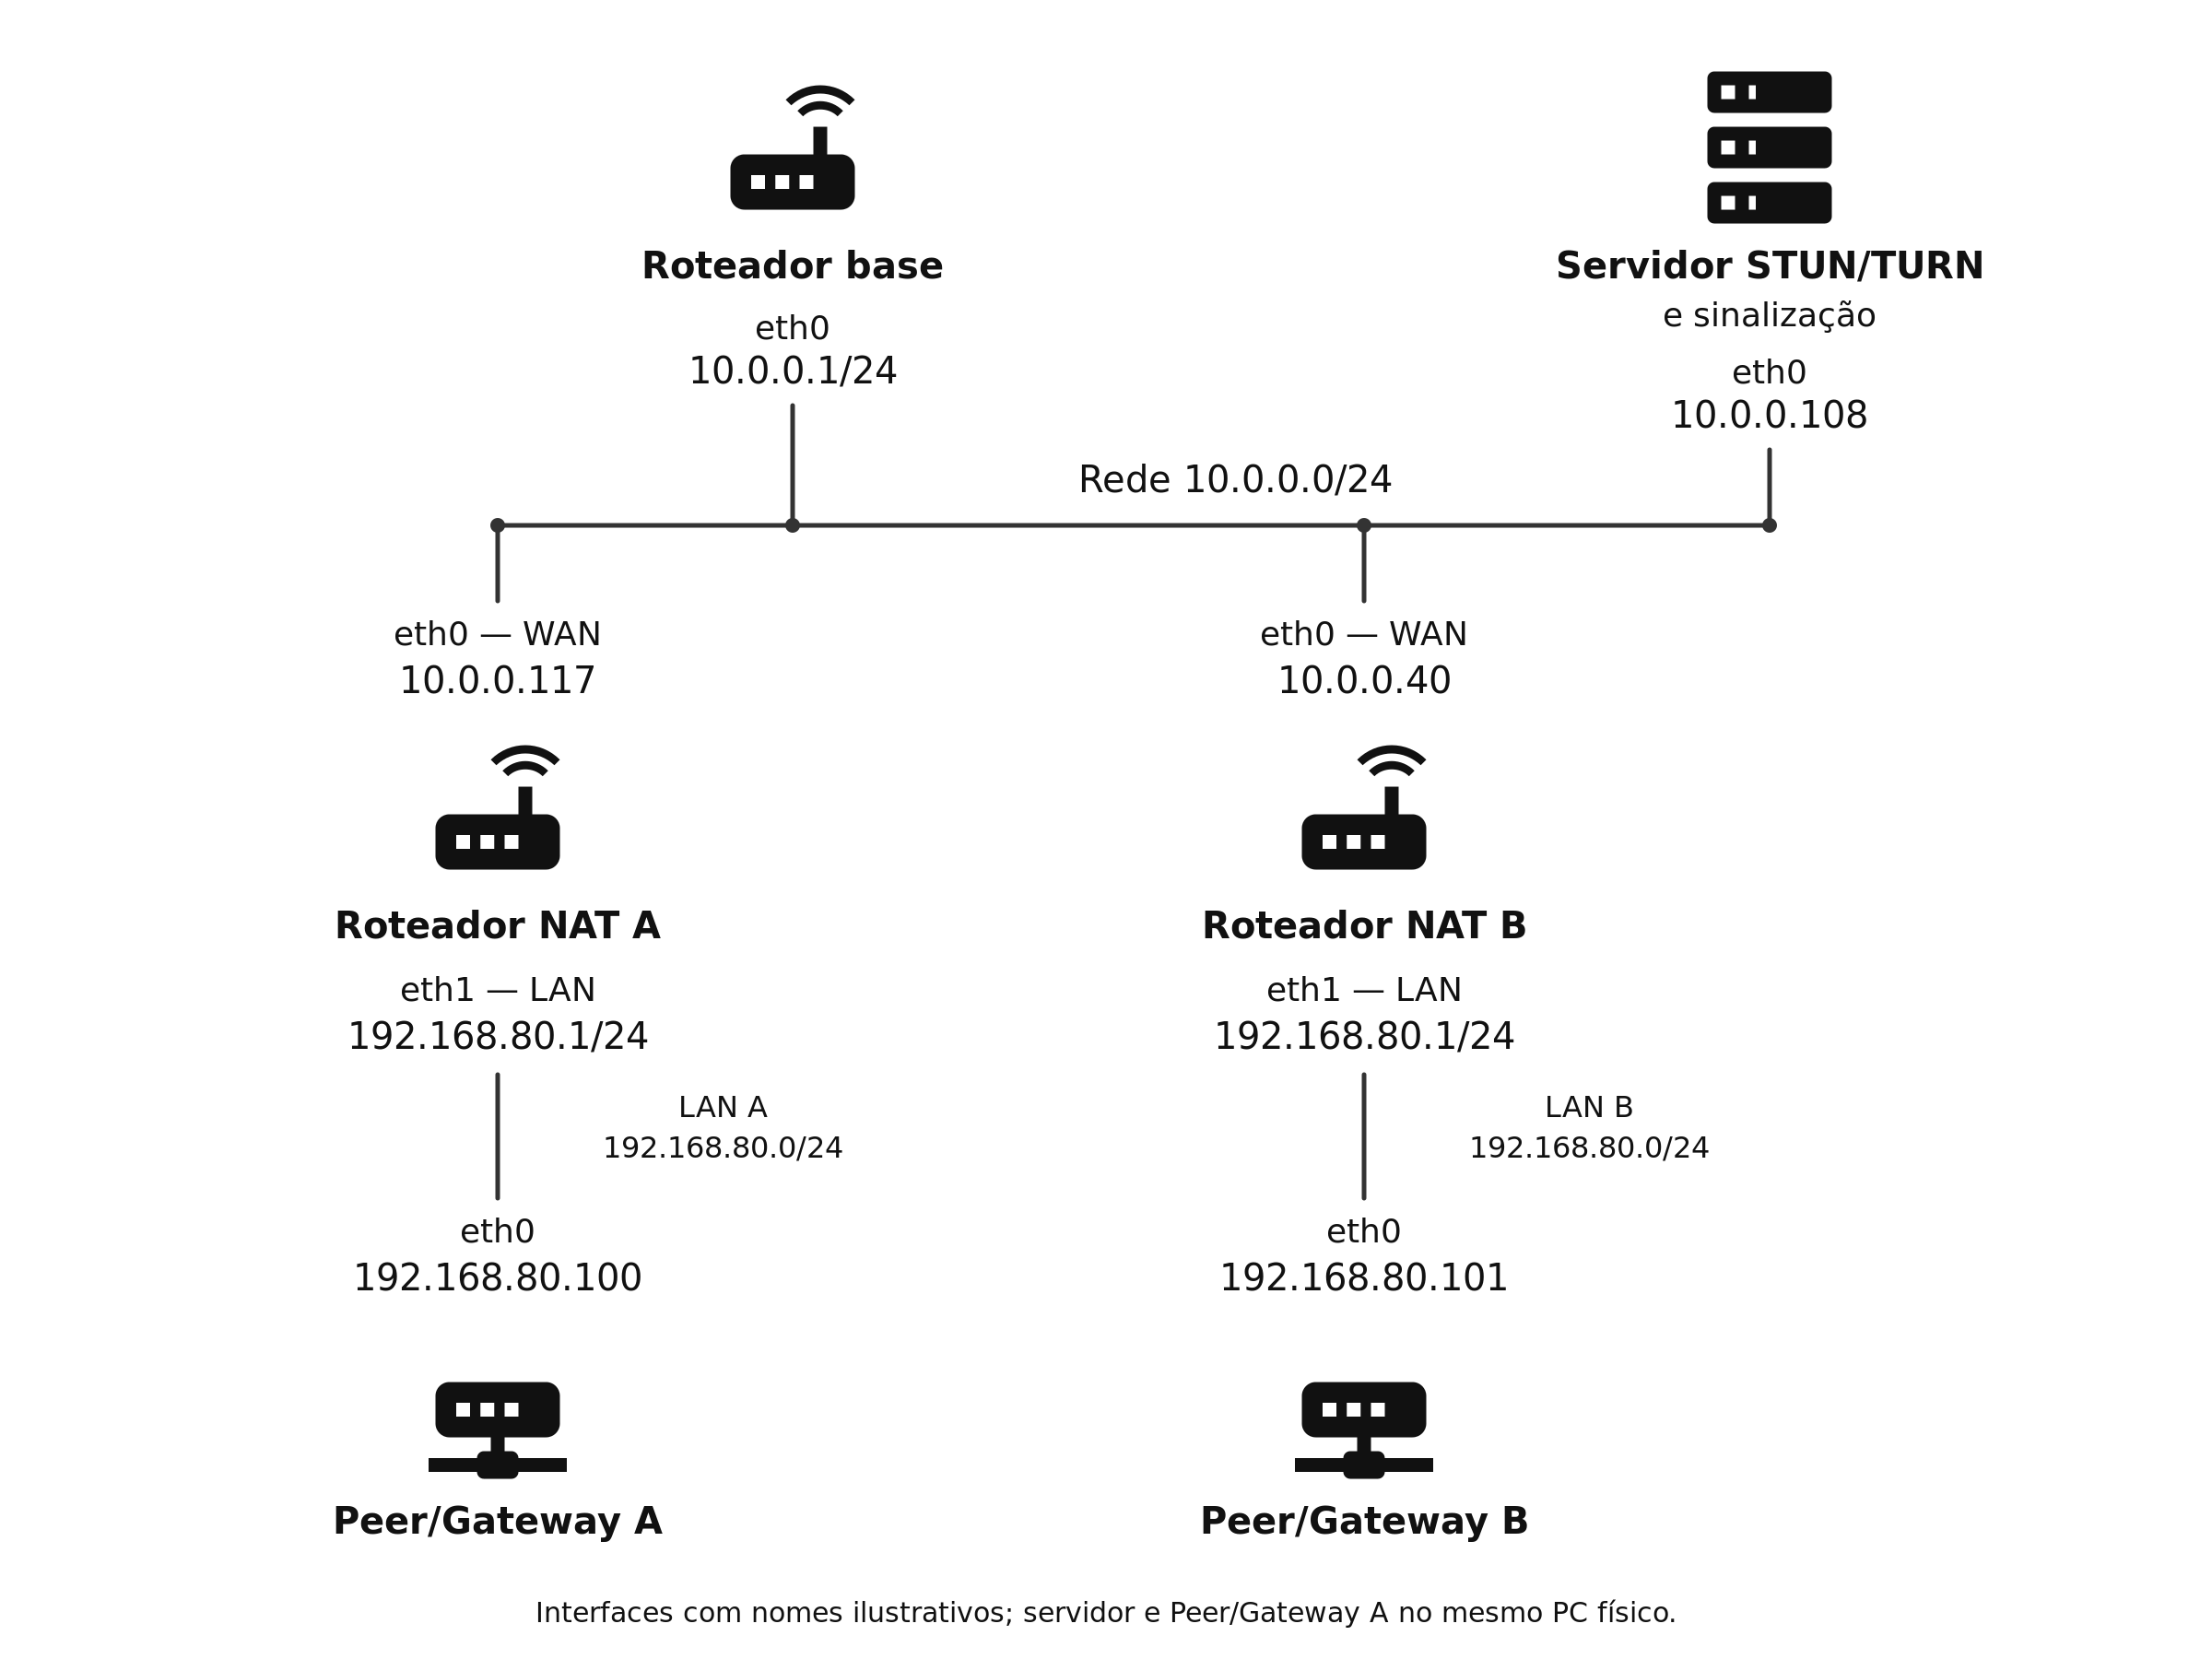
\includegraphics[width=0.7\textwidth]{fig/results/physical/physical_topology.png}
    \caption{Topologia física com roteadores da DATACOM.}
    \label{fig:physical_topology}
\end{figure}

O primeiro computador acumula duas funções: executar o \textit{peer} A e hospedar os serviços auxiliares. Sua interface Ethernet conecta o \textit{peer} A à LAN do roteador A, e sua interface Wi-Fi conecta o servidor à rede do roteador base, com o endereço \texttt{10.0.0.108}. Nesse servidor, o \texttt{coturn} disponibiliza STUN/TURN por UDP na porta 3478, e o serviço de sinalização utiliza TCP na porta 5555. O segundo computador executa o \textit{peer} B, conectado à LAN do roteador B.

Para separar as funções do primeiro computador, a interface Ethernet do \textit{peer} A é movida para um \textit{network namespace} próprio, cuja rota padrão aponta para o roteador A. Sem essa separação, a pilha de rede local encaminharia diretamente o tráfego entre o \textit{peer} A e o servidor, hospedado no mesmo computador, sem passar pelo roteador NAT. Diferentemente do ambiente \texttt{PatchBay}, nesse caso o \textit{namespace} isola uma interface física, e o encaminhamento e a tradução de endereços ocorrem nos roteadores externos.

Um \textit{script} organiza a execução, com papéis distintos para os dois computadores. No papel A, o \textit{script} prepara os serviços auxiliares, o \textit{namespace} e a aplicação geradora de dados. No papel B, o \textit{script} inicia o \textit{peer} remoto e um serviço TCP de \textit{echo}.

O \textit{script} também inicia capturas de pacotes nas interfaces utilizadas pelo \textit{peer} A, pelo servidor e pelo \textit{peer} B. Os arquivos PCAP e os \textit{logs} dos processos são armazenados por execução, o que permite relacionar a negociação ICE, o estabelecimento da conexão QUIC e a comunicação entre os \textit{gateways}. A Seção~\ref{sec:physical_results} apresenta os resultados obtidos nesse ambiente.
